\section{Introduction}
\label{sec:introduction}

Vision-language-action (VLA) policies are increasingly evaluated by asking a robot to perform the same task under counterfactual instructions. For relational placement, a natural test is to hold the scene fixed, replace \emph{left} with \emph{right}, and compare task success. A large LEFT/RIGHT gap is then tempting to read as a language-grounding failure: the model understood one direction but not the other, or vision overrode language. This interpretation has practical consequences. It directs effort toward stronger language conditioning, counterfactual relabeling, or steering at inference time~\cite{fang2026cag,glossop2025cast,chen2026steerable}.

The success gap, however, combines several questions. The instruction must alter control; the change must be oriented toward the requested relation; the robot must execute a feasible grasp and transport trajectory; and the final state must cross a binary task boundary. A policy can pass the first two steps but fail the last two because one side of a particular layout is harder to reach. The reverse mistake is also possible: a policy can react predictably to the literal tokens LEFT and RIGHT without preserving the same physical goal when the linguistic reference frame is inverted. Neither case is identified by a single binary contrast.

We audit this inference with two kinds of matched intervention. First, we compare canonical LEFT and RIGHT prompts under identical simulator and sampling state. Across 324 pairs, 253 endpoint pairs are ordered in the token-associated direction, while all 324 pairs execute different action sequences. Second, we express the same physical relation from the other object's reference frame: ``cube left of bowl'' becomes ``bowl right of cube,'' and conversely. Under this reference inversion, $\pi_{0.5}$ does not preserve the canonical directional endpoint separation. Canonical token sensitivity is therefore not sufficient evidence of relation-level generalization.

Fig.~\ref{fig:screening} reports all eight completed checkpoint--arena rows before any diagnostic narrowing. Binary directional disparity varies sharply by checkpoint and arena. Later intervention figures therefore show their registered checkpoint subsets, and geometric equalization claims are restricted to rows that pass the relevant endpoint-redirection control. Within those subsets, we intervene on the scene while keeping prompts, policies, robot, cameras, controller, and seeds fixed. Position reflection reverses the placement advantage in three checkpoints; a seven-position displacement sweep grades it continuously; and a registered symmetric scene sharply reduces it across the qualifying DROID/RoboLab checkpoints.

Our contribution is an evaluation argument supported by controlled experiments:
\begin{itemize}
    \item We show that canonical LEFT/RIGHT task success does not isolate language grounding. Action change, endpoint orientation, continuous goal progress, and binary completion must be measured separately.
    \item We introduce a reference-inversion control and show that canonical-token response need not transfer when the same relation is expressed from the other object's frame.
    \item We provide matched reflection, graded displacement, role, start-side, and symmetric-scene interventions showing that scene configuration can reverse or largely remove a directional completion gap without changing the evaluated policy.
\end{itemize}
\begin{figure*}[t]
  \centering
  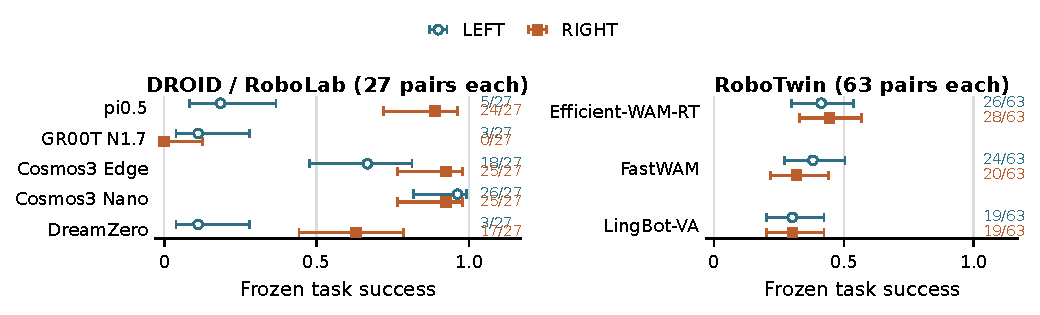
\includegraphics[width=0.98\textwidth]{figures/checkpoint_screen.pdf}
  \caption{\textbf{Directional task success varies across all eight completed checkpoint--arena rows.}
  Points show marginal LEFT and RIGHT success with 95\% Wilson intervals. DROID/RoboLab uses 27 matched pairs per row and RoboTwin 63; their tasks and frozen predicates differ and are never pooled. This screen is separate from later intervention cohorts, and its intervals are descriptive rather than matched-pair tests.}
  \label{fig:screening}
\end{figure*}
